% Graphic for TeX using PGF
% Title: /home/di3go/workspace/t02-core-musa/doc/architecture/dia_projects/diagramas_de_classe/ula.dia
% Creator: Dia v0.97.2
% CreationDate: Mon Dec  8 21:41:52 2014
% For: di3go
% \usepackage{tikz}
% The following commands are not supported in PSTricks at present
% We define them conditionally, so when they are implemented,
% this pgf file will use them.
\ifx\du\undefined
  \newlength{\du}
\fi
\setlength{\du}{15\unitlength}
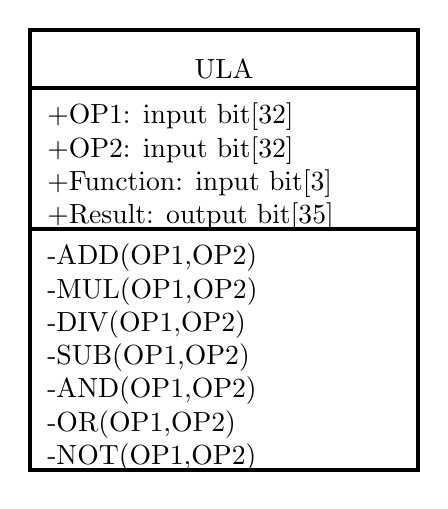
\begin{tikzpicture}
\pgftransformxscale{1.000000}
\pgftransformyscale{-1.000000}
\definecolor{dialinecolor}{rgb}{0.000000, 0.000000, 0.000000}
\pgfsetstrokecolor{dialinecolor}
\definecolor{dialinecolor}{rgb}{1.000000, 1.000000, 1.000000}
\pgfsetfillcolor{dialinecolor}
\pgfsetlinewidth{0.100000\du}
\pgfsetdash{}{0pt}
\definecolor{dialinecolor}{rgb}{1.000000, 1.000000, 1.000000}
\pgfsetfillcolor{dialinecolor}
\fill (-9.998130\du,-11.940600\du)--(-9.998130\du,-10.540600\du)--(-0.643130\du,-10.540600\du)--(-0.643130\du,-11.940600\du)--cycle;
\definecolor{dialinecolor}{rgb}{0.000000, 0.000000, 0.000000}
\pgfsetstrokecolor{dialinecolor}
\draw (-9.998130\du,-11.940600\du)--(-9.998130\du,-10.540600\du)--(-0.643130\du,-10.540600\du)--(-0.643130\du,-11.940600\du)--cycle;
% setfont left to latex
\definecolor{dialinecolor}{rgb}{0.000000, 0.000000, 0.000000}
\pgfsetstrokecolor{dialinecolor}
\node at (-5.320630\du,-10.990600\du){ULA};
\definecolor{dialinecolor}{rgb}{1.000000, 1.000000, 1.000000}
\pgfsetfillcolor{dialinecolor}
\fill (-9.998130\du,-10.540600\du)--(-9.998130\du,-7.140600\du)--(-0.643130\du,-7.140600\du)--(-0.643130\du,-10.540600\du)--cycle;
\definecolor{dialinecolor}{rgb}{0.000000, 0.000000, 0.000000}
\pgfsetstrokecolor{dialinecolor}
\draw (-9.998130\du,-10.540600\du)--(-9.998130\du,-7.140600\du)--(-0.643130\du,-7.140600\du)--(-0.643130\du,-10.540600\du)--cycle;
% setfont left to latex
\definecolor{dialinecolor}{rgb}{0.000000, 0.000000, 0.000000}
\pgfsetstrokecolor{dialinecolor}
\node[anchor=west] at (-9.848130\du,-9.840600\du){+OP1: input bit\ensuremath{[}32\ensuremath{]}};
% setfont left to latex
\definecolor{dialinecolor}{rgb}{0.000000, 0.000000, 0.000000}
\pgfsetstrokecolor{dialinecolor}
\node[anchor=west] at (-9.848130\du,-9.040600\du){+OP2: input bit\ensuremath{[}32\ensuremath{]}};
% setfont left to latex
\definecolor{dialinecolor}{rgb}{0.000000, 0.000000, 0.000000}
\pgfsetstrokecolor{dialinecolor}
\node[anchor=west] at (-9.848130\du,-8.240600\du){+Function: input bit\ensuremath{[}3\ensuremath{]}};
% setfont left to latex
\definecolor{dialinecolor}{rgb}{0.000000, 0.000000, 0.000000}
\pgfsetstrokecolor{dialinecolor}
\node[anchor=west] at (-9.848130\du,-7.440600\du){+Result: output bit\ensuremath{[}35\ensuremath{]}};
\definecolor{dialinecolor}{rgb}{1.000000, 1.000000, 1.000000}
\pgfsetfillcolor{dialinecolor}
\fill (-9.998130\du,-7.140600\du)--(-9.998130\du,-1.340600\du)--(-0.643130\du,-1.340600\du)--(-0.643130\du,-7.140600\du)--cycle;
\definecolor{dialinecolor}{rgb}{0.000000, 0.000000, 0.000000}
\pgfsetstrokecolor{dialinecolor}
\draw (-9.998130\du,-7.140600\du)--(-9.998130\du,-1.340600\du)--(-0.643130\du,-1.340600\du)--(-0.643130\du,-7.140600\du)--cycle;
% setfont left to latex
\definecolor{dialinecolor}{rgb}{0.000000, 0.000000, 0.000000}
\pgfsetstrokecolor{dialinecolor}
\node[anchor=west] at (-9.848130\du,-6.440600\du){-ADD(OP1,OP2)};
% setfont left to latex
\definecolor{dialinecolor}{rgb}{0.000000, 0.000000, 0.000000}
\pgfsetstrokecolor{dialinecolor}
\node[anchor=west] at (-9.848130\du,-5.640600\du){-MUL(OP1,OP2)};
% setfont left to latex
\definecolor{dialinecolor}{rgb}{0.000000, 0.000000, 0.000000}
\pgfsetstrokecolor{dialinecolor}
\node[anchor=west] at (-9.848130\du,-4.840600\du){-DIV(OP1,OP2)};
% setfont left to latex
\definecolor{dialinecolor}{rgb}{0.000000, 0.000000, 0.000000}
\pgfsetstrokecolor{dialinecolor}
\node[anchor=west] at (-9.848130\du,-4.040600\du){-SUB(OP1,OP2)};
% setfont left to latex
\definecolor{dialinecolor}{rgb}{0.000000, 0.000000, 0.000000}
\pgfsetstrokecolor{dialinecolor}
\node[anchor=west] at (-9.848130\du,-3.240600\du){-AND(OP1,OP2)};
% setfont left to latex
\definecolor{dialinecolor}{rgb}{0.000000, 0.000000, 0.000000}
\pgfsetstrokecolor{dialinecolor}
\node[anchor=west] at (-9.848130\du,-2.440600\du){-OR(OP1,OP2)};
% setfont left to latex
\definecolor{dialinecolor}{rgb}{0.000000, 0.000000, 0.000000}
\pgfsetstrokecolor{dialinecolor}
\node[anchor=west] at (-9.848130\du,-1.640600\du){-NOT(OP1,OP2)};
\end{tikzpicture}
